\documentclass{standalone}
\usepackage{tikz}
\begin{document}
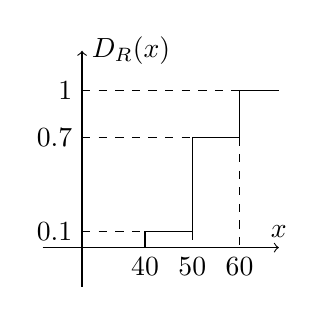
\begin{tikzpicture}[scale=2]
    \draw[->](-0.25,0)--(1.25,0)node[above]{$x$};
    \draw[->](0,-0.25)--(0,1.25)node[right]{$D_R(x)$};
    \draw (0.4,0)node[below]{$40$}--(0.4,0.1)--(0.7,0.1)--(0.7,0.7)--(1,0.7)--(1,1)--(1.25,1);
    \draw[dashed](0,0.1)node[left]{$0.1$}--(0.4,0.1);
    \draw[dashed](0,0.7)node[left]{$0.7$}--(0.7,0.7);
    \draw[dashed](0,1)node[left]{$1$}--(1,1);
    \draw[dashed](0.7,0.1)--(0.7,0)node[below]{$50$};
    \draw[dashed](1,0.7)--(1,0)node[below]{$60$};
\end{tikzpicture}
\end{document}